\chapter*{Заключение}
\addcontentsline{toc}{chapter}{Заключение}
\label{chapter:summary}

\section*{Резултати}
\addcontentsline{toc}{section}{Резултати}

Считаме, че представеният научен труд изпълнява поставената цел и задачи. В този раздел ще обобщим постигнатите резултати и как те се отнасят към изпълнението на споменатите цел и задачи. В хода на изследването бяха постигнати всичките шест задачи и резултатите бяха публикувани в престижни международни списания и представени на големи конференции в България и в чужбина. Най-важните от тях са обобщени както следва:

\paragraph{Резултат 1.} Основният резултат на дисертацията е създаването на концептуален модел на областта на публикуването на знание за биологичното разнообразие и логическото му формализиране му под формата на онтологията OpenBiodiv-O. OpenBiodiv-O дава възможност за свързване на знанията за биоразнообразието въз основа на научни публикации. OpenBiodiv-O е базата на Свързаните Отворени Данни OpenBiodiv-LOD. Чрез разработването на онтология, насочена към биологичната таксономия, осигуряваме онтология, която запълва празнините между онтологиите за ресурси от биологичното разнообразие като Darwin-SW и онтологиите за семантично публикуване като SPAR. Освен това считаме, че е правилно да се моделира самият таксономичен процес, а не някакво конкретно състояние на знанието, тъй като въпросният процес далеч не е завършил и няма изгледи да завърши в скоро бъдеще. Този резултат е подробно дискутиран в глава~\ref{chapter-ontology} и в \cite{senderov_openbiodiv-o:_2018} и изпълнява Задача 1. Сорс кодът на онтологията е достъп под \href{https://github.com/pensoft/openbiodiv-o}{github.com/pensoft/openbiodiv-o}. На дадения етап, покритието на онтологията на различните типове ресурси е достатъчно, за да може тя да бъде основата за създаването на LOD. В този смисъл тя е завършена. От друга страна добавяне на класове и свойства за нови типове данни за биоразнообразието е възможно и желателно.

\paragraph{Резултат 2.} Друг резултат на тезата е създаването на софтуерната архитектура на OpenBiodiv, очертана в глава~\ref{chapter-openbiodiv} и \cite{senderov_open_2016}. Този резултат отговаря на Задача 2.

\paragraph{Резултат 3.} Третият резултат на дисертацията е създаването на Свързани Отворени Данни, OpenBiodiv-LOD, състоящи се от трансформирани в RDF и интегрирани в база данни твърдения за биоразнообразието. Твърденията са извлечени от XML на научни статии, публикувани от Пенсофт, XML таксономични дискусии, публикувани от Плаци, и CSV дъмп на таксономичният гръбнак на GBIF. OpenBiodiv-LOD е достъпен под \href{http://graph.openbiodiv.net}{\url{graph.openbiodiv.net}} и е описан в глава~\ref{chapter-lod}. Този резултат отговаря на Задача 3. Свързаните отворени данни, подобно на онтологията, вече представляват солиден ресурс за биолозите, тъй като включват информация от повечето статии, публикувани от Пенсофт и Плаци и наброяват над 600 милиона трипъла. Подобно на онтологията, те следва да бъдат разширявани.

\paragraph{Резултат 4.} За да подпомогне създаването на Свързаните Отворени Данни, е разработен софтуерен пакет за средата за програмиране R, RDF4R. RDF4R дава възможност за манипулиране на RDF в R и улеснява за трансформирането на научни публикации от полу-структуриран XML формат в структуриран семантичен RDF. Този резултат е обсъден в глава~\ref{chapter-rdf4r} и \cite{senderov_online_2016} и изпълнява Задача~4. Пакетът е достъпен онлайн като свободен софтуер под \href{http://github.com/pensoft/rdf4r}{github.com/pensoft/rdf4r}. Освен това допълнителен изходен код (не-оптимизиран), описващ XML схемите на Пенсофт и Плаци и работещ в тандем с RDF4R за конвертиране на XML в RDF може да бъде намерен под \href{http://github.com/pensoft/ropenbio}{github.com/pensoft/ropenbio}. Тъй като пакетът беше използван успешно за създаването на LOD, той може да се счита за завършен. Както всеки един софтуерен пакет, обаче, той би следвало да бъде поддържан и развиван. Детайли относно насоките за развитието му са поместени в следващия раздел.

\paragraph{Резултат 5.} Механизмите за преобразуване на полу-структуриран XML в RDF се допълват от процеси за работа, които позволяват обогатяването на XML статии, публикувани от Пенсофт, чрез автоматично импортиране на данни от основните международни хранилища за данни за биологичното разнообразие: BOLD, GBIF, iDigBio , както и PlutoF. Освен това, благодарение на това дисертационно усилие е възможно автоматично да се създадат ръкописи от метаданни, кодирани в Ecological Metadata Language (EML). Обсъждането на тези автоматизирани работни процеси -- автоматично генериране на data papers и автоматичен импорт на occurrence records - се извършва в глава~\ref{chapter-case-study}. Този резултат изпълнява Задача 5.

\paragraph{Резултат 6.} За да допълним създаването на OpenBiodiv-LOD, ние разработихме уеб сайт който използва гр\'{а}фа от знания \href{http://openbiodiv.net}{openbiodiv.net}, съдържащ семантична търсачка и приложения. Уебсайтът е обсъден в глава~\ref{chapter-webportal} и изпълнява Задача 6. Уебсайтът е все още в бета-версия. Функционалността, която работи отлично е семантичната търсачка. За някои основни типове данни има създадени темплейти за визуализация. Въпреки всичко, сайтът не може да се счита за завършен и повечето потребители на системата използват езика за SPARQL за търсене.

\section*{Изводи и бъдещи насоки}
\addcontentsline{toc}{section}{Обобщителна дискусия на резултатите и бъдещи насоки}

Важен извод, който може да се направи като обобщение на постигнатите резултати е, че е възможно използването на семантичен граф за интегрирането на голям обем от данни за биологичното разнообразие. Неочаквано ни се отдаде възможност да илюстрираме мощта на графа при анализа на щетите от трагичния пожар в Museu Nacional в Рио де Жанейро. Освен това илюстрирахме, че е възможно да се напишат сравнително прости логически изводи, позволяващи проверка на валидността на дадено таксономично име.

Поради значителния размер на данните установихме, че макар и използването на семантичен граф да е възможно, някои от първоначално избраните технологии се оказаха неприложими или трудно приложими. Извършихме наблюдението (вж. глава~\ref{chapter-lod}), че практическото приложение на пълния логически модел OWL е трудно, поради проблеми с бързодействието. Вместо него се спряхме на по-маломощната, но по-бърза RDFS. Друго наблюдение, което направихме е, че макар и програмната среда R да ни даде известни предимства при бързото създаване на прототипа на системата, при увеличаването на сложността на програмния код, необходимо при реално-съществуващата система за покриване на всички частни случаи, език с динамични типове като R създава главоболия при дебъгинг. Същевременно останахме впечатлени от мощния инструментариум на функционалното програмиране, който R предоставя.

Основна трудност се оказа дизамбигуацията на ресурси като имена на автори или таксономични имена. Във функционалния дизайн на пакета RDF4R заложихме модули, които позволяват при търсенето на идентификатор за даден ресурс да вмъкнем списък от функции/ правила за неговата дизамбигуация. Въпреки това имахме само ограничен успех с дизамбигуацията на базата на правила и по тази причина в производствената система тя е изключена към момента.

Имайки предвид тези и други ``поуки'' бъдещето развитие на проекта OpenBiodiv може да се очертае по следния не непременно изчерпателен начин: 

\begin{enumerate}
    \item Като непосредствени цели да разширят LOD и онтологията с нови типове данни и нови източници на данни, използвайки съществуващия фреймуърк. Такива данни са напр. геномните данни, данните са местонаходища на видове, (био-)географски данни, визуални данни, описателни данни и пр.
    \item Да се търси още по-тясна интеграция с други съществуващи хранилища за данни за биоразнообразието освен GBIF. Напр. BioImages, iNaturalist, BOLD, и т.н.
    \item Като по-дългосрочна задача да се изследва преминаването от семантичен граф към технология, където машината за извод е разграничена от семантичния граф като WikiData или Neo4j. Освен увеличеното бързодействие, това ще даде допълнителна гъвкавост на проекта като например позволи използването на машини за извод различни от RDF-базирането като напр. Euler.
    \item Да бъде продължена разработката на системния софтуер с още по-широко приложение на функционалното програмиране и портирането му към фунцкионален език като напр. Haskell или O'Caml.
    \item Да бъде изследван проблемът за дизамбигуацията и сродните проблеми за named entity recognition на интересни ресурси от биоразнообразието, както и различни задачи от разпознаването на образи, от гледната точка на машинното обучение.
    \item Разширяване на уебсайта на системата с повече темплейти и нови приложения.
\end{enumerate}

\section*{Основни научни и научно-приложни приноси}
\addcontentsline{toc}{section}{Основни научни и научно-приложни приноси}

Резултатите, дискутирани в предишните два раздела, обуславят следните научни и научно-приложни приноси:

\begin{enumerate}
    \item Научен принос: създаване на онтология и формален модел на областта на публикуване на знание за биологичното разнообразие.
    \item Научно-приложен принос: анализ на източниците на информация и създаване на OpenBiodiv-LOD.
    \item Научно-приложен принос: имплементация на софтуерните модули на OpenBiodiv.
\end{enumerate}

Нашата онтология запълва уникалната ниша между библиографски онтологии като SPAR и онтологии за биоразнообразието като Darwin-SW и като такава без съмнение е от голям научен интерес за общността на информатиката на биоразнообразието. Работата има и сериозен научно-приложен характер, като в допълнение на онтологията като предоставя и свързани отворени данни, използващи онтологията, както и програмно обезпечение за потребителите и разработчиците на системата.

\section*{Списък с публикации}
\addcontentsline{toc}{section}{Списък с публикации}

\subsection*{Публикации в международни научни списания}
\addcontentsline{toc}{subsection}{Публикации в международни научни списания}

\begingroup
\newcounter{count}
\setcounter{count}{99}
\defcounter{maxnames}{\value{count}}%

\begin{enumerate}
\item \longfullcite{senderov_open_2016}. Поне 3 уникални цитата от \cite{franz_increase_2018}, \cite{ordynets_aphyllophoroid_2017} и \cite{burt_origin_2017}.
\item \longfullcite{sarah_faulwetter_emodnet_2016}. Уникален цитат от \cite{pyron_21st_2018}.
\item \longfullcite{cardoso_species_2016}. Индексация в WoS SCOPUS, както и в SJR $0.465$. Поне 4 уникални цитата от \cite{bachman_quantifying_2018}, \cite{lin_draft_2017}, \cite{li_genomic_2017} и \cite{milano_conservazione_2017}.
\item \longfullcite{senderov_online_2016}. Уникален цитат от \cite{ordynets_aphyllophoroid_2017}.
\item \longfullcite{penev_strategies_2017} Поне 8 уникални цитата от \cite{tennant_multi-disciplinary_2017}, \cite{marwick_standard_2017},  \cite{kissling_towards_2018},  \cite{mathieu_egrowth:_2018}, \cite{__2018}, \cite{__2017}, \cite{filippova_biodiversity_2017} и  \cite{__2017-1}.
\item \longfullcite{penev_arpha-biodiv:_2017} 
\item \longfullcite{arriaga-varela_review_2017}. Индексация в WoS IF $1.079$, Q3 SCOPUS, SJR $0.533$.
\item \longfullcite{senderov_openbiodiv-o:_2018} Индексация в WoS IF $1.6$, Q3 SCOPUS, SJR $0.952$. Поне 3 уникални цитата от \cite{michel_modelling_2018}, \cite{page_ozymandias:_2018} и \cite{page_liberating_2018}.
\end{enumerate}
\endgroup

Представен е списък с публикации, свързани с дисертацията. Изброените статии са публикувани без изключение в четири международни научни списания: пет статии в Research Ideas and Outcomes, една статия в ZooKeys (WoS IF $1.079$, Q3 SCOPUS, SJR $0.533$), една статия в Biodiversity Data Journal (WoS SCOPUS, SJR 0.465) и една статия в Journal of Biomedical Semantics (WoS IF $1.6$, Q3 SCOPUS, SJR $0.952$). Общият брой цитати, които кандидатът е натрупал, изключвайки самоцитати е най-малко 20, като конкретните цитиращи статии са посочени в списъка по горе. Общият брой на натрупаните цитати, включително самоцитати и цитати на работа извън обхвата на дисертацията, е най-малко 48 (Google Наука).

[1] е ранна версия на въведението, както и на глава~\ref{chapter-openbiodiv} и съдържа труд по Задача 2 (Архитектура). Текстовете на публикациите [2, 3, 5, 6, 7] не са част от текста на дисертацията дословно, но съдържат труд по Задача 5 (Методи за работа). Представените в тези публикации идеи са в голяма степен включени в глава~\ref{chapter-case-study}, чиито текстови гръбнак се формира от публикация [4]. [8] е най-важната публикация в рамките на тази дисертация и е публикувана във реномираното списание Journal of Biomedical Semantics. [8] съставлява съдържанието на глава~\ref{chapter-ontology} и е основната част от работата, изпълняваща Задача 1 (Онтология). Статията беше на заглавната страница на JBS в продължние на няколко месеца (фиг. \ref{fig:jbs-featured}). Глава~\ref{chapter-lod} и глава~\ref{chapter-rdf4r}, които формират Задачи 3, 4, се подготвят като ръкописи в международни списания. Освен това софтуерната библиотека RDF4R, описана в глава~\ref{chapter-rdf4r}, се подготвя да бъде изпратена в хранилището с отворен код rOpenSci\footnote{``We build software with a community of users and developers, and educate scientists about transparent research practices.'' \url{https://ropensci.org/}}.



\begin{figure}
\centering
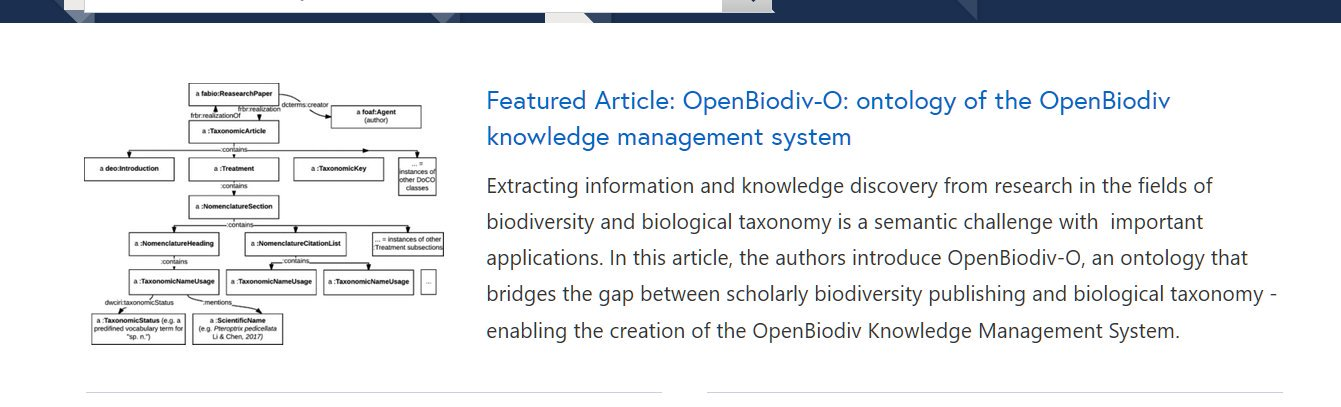
\includegraphics[width=\textwidth]{Figures/JBS-featured.jpg}
\decoRule
\caption{Статията относно OpenBiodiv-O е на началната страница на Journal of Biomedical Semantics.}
\label{fig:jbs-featured}
\end{figure}

\section*{Апробация на резултатите}
\addcontentsline{toc}{section}{Апробация на резултатите}

\subsection*{Доклади пред научен семинар на ПНЗ}
\addcontentsline{toc}{subsection}{Доклади пред научен семинар на ПНЗ}

\begin{enumerate}
    \item Доклад пред научен семинар на ИБЕИ на БАН на 26.10.2015 г. (“Публикуване, визуализация и разпространение на първични и геномни данни за биологичното разнообразие на основата на открита система за управление на информацията”).
    \item Доклад пред научен семинар в ИИКТ на БАН на 31.03.2016 г. (Open Biodiversity Knowledge Management System)
    \item Доклад пред научен семинар на ИИКТ на БАН за 23.03.2018 г. (OpenBiodiv: a knowledge-based system of biodiversity information)
\end{enumerate}

\subsection*{Доклади пред научно мероприятие в чужбина или пред международно научно мероприятие у нас}
\addcontentsline{toc}{subsection}{Доклади пред научно мероприятие в чужбина или пред международно научно мероприятие у нас}

\begin{enumerate}
    \item Доклад пред международния симпозиум EU BON в София на 23.03.2016 г. (The Data Publishing Toolkit at EU BON: Automated creation of data papers, data and text integrated publishing via the ARPHA Publishing Platform.)
    \item Доклад по време на работната среща на BIG4 в Хавраники, Чехия на 03.06.2016 г. (Project Progress Report (OBKMS))
    \item Доклад по време на работната среща на BIG4 в Хавраники, Чехия на 03.06.2016 г. (Modern Methods of Systematic Research and the BOLD Algorithm)
    \item Уеб-базиран доклад (уебинар) пред международна аудитория в рамките на семинар на iDigBio на 16.07.2016 г. (Online direct import of specimen records from iDigBio instrastructure into taxonomic manuscripts)
    \item Доклад по време на работната среща на BIG4 в Копенхаген на 14.10.2016 г. (Midterm Progress Report)
    \item Доклад на международия симпозиум TDWG 2016 в Санта Клара де Сан Карлос от 5. до 9.12.2016 г. (Streamlining the Flow of Taxon Occurrence Data Between a Manuscript and Biological Databases)
    \item Доклад на международия симпозиум TDWG 2016 в Санта Клара де Сан Карлос от 5. до 9.12.2016 г. (The Open Biodiversity Knowledge Management System: A Semantic Suite Running on top of the Biodiversity Knowledge Graph)
    \item Доклад на международия симпозиум TDWG 2016 в Санта Клара де Сан Карлос от 5. до 9.12.2016 г. (Demonstrating the Prototype of the Open Biodiversity Knowledge Management System)
    \item Доклад на международия симпозиум TDWG 2016 в Санта Клара де Сан Карлос от 5. до 9.12.2016 г. (Creation of Data Paper Manuscripts from Ecological Metadata Language (EML))
    \item Уеб-базиран доклад пред междуродния семинар на работната група по семантични технология към Университета Вандербилт (Тенеси, САЩ) на 20.02.2017 г. (Open Biodiversity Knowledge Management System)
    \item Доклад на европейската конференция на биосистематиците, BioSyst.eu 2016 на 15.08.2017 г. (The OpenBiodiv Knowledge System: The Future of Access to Biodiversity Knowledge)
    \item Доклад на международия симпозиум TDWG 2017 в Отава, Канада от 1. до 6.10.2017 г. (OpenBiodiv Computer Demo: an Implementation of a Semantic System Running on top of the Biodiversity Knowledge Graph)
    \item Доклад на международия симпозиум TDWG 2017 в Отава, Канада от 1. до 6.10.2017 г. (OpenBiodiv: an Implementaion of a Semantic System Running on top of the Biodiversity Knowledge Graph)
    \item Постер на международия симпозиум TDWG 2017 в Отава, Канада от 1. до 6.10.2017 г. (OpenBiodiv: an Implementaion of a Semantic System Running on top of the Biodiversity Knowledge Graph)
    \item Доклад по време на работната среща на BIG4 в Ла Палма, Испания от 30. окт. до 3 ноем. 2017 г. (Midterm Progress Report)
    \item Доклад пред научен семинар на групата по биоинформатика (група Ронкуист) в Кралския природо-научен музей в Стокхолм на 29.11.2017 г.
\end{enumerate}





